%************************************************
\chapter{Developer Guide}\label{ch:developer_guide} % $\mathbb{ZNR}$
%************************************************

To allow further development of the application, the design will be described in a top down approach, starting from a high level overview and going into details only where necessary.

\section{Architectural overview}
\label{sec:architectural overview}

The application was developed taking into account the principle of separating program logic from interface design. To support this approach the \acf{MVP} design pattern was utilized.

\begin{figure}[H]
\begin{center}
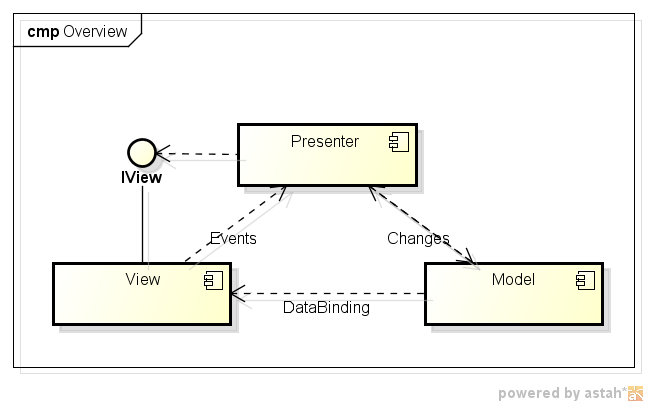
\includegraphics[width=\textwidth]{gfx/architecture_overview.png}
\caption{Architecture overview with \ac{MVP}}
\label{fig:architecture_overview}
\end{center}
\end{figure}

This separation allows the view to be decoupled from the presenter and the model, as the presenter only communicates with the view over a well-defined interface (\texttt{IView}), whereas the view communicates only with provided methods from the presenter.

When changes occur in the model, the view will be notified via the data-binding mechanism of WinForms.
% TODO put reference.

The implementation of this pattern splits the application into two projects:
\begin{description}
\item[UserInterface:] Hosts the graphical user interface and all code related to changing the appearance of the application.
\item[ApplicationLogic:] Hosts the \texttt{presenter} and the \texttt{model} component of the diagram.
\end{description}

These two packages will be described in-depth:

\section{UserInterface}
\label{sec:user_interface}

The user interface package holds the WinForms representation of a possible \ac{GUI}\footnote{It is a \textit{possible} \ac{GUI}, as  another one should - due to the decoupling of view and logic - be easily realisable by implementing the \texttt{interfaces} of the \texttt{ApplicationLogic} package.}.

The \texttt{MainWindow} holds a reference to the \texttt{presenter} and the \texttt{model}.

The \texttt{presenter} handles all events that need more logic than just changing the view's appearance\footnote{E.g. enabling/disabling buttons, changing the color of fields, showing a new window.}

The \texttt{model}-reference is used to set-up the data-binding in the application:

\begin{lstlisting}[caption=Data Binding of \texttt{view} and \texttt{model}]
private void SetUpDataBindings()
        {
            stockItemsListBox.DataSource = _Model.StockItems;
            stockItemsListBox.DisplayMember = "Name";

            /*
             * The datasourceupdatemode is set to "Never".
             * This leads to the ability to enforce the use of the presenter to update the values in the model.
             * This way the validation errors can be handled by the presenter thus leading to better seperation of concerns.
             */
            stockCodeTextBox.DataBindings.Add("Text", _Model.StockItems, "StockCode", false, DataSourceUpdateMode.Never);
            itemNameTextBox.DataBindings.Add("Text", _Model.StockItems, "Name", false, DataSourceUpdateMode.Never);
            supplierNameTextBox.DataBindings.Add("Text", _Model.StockItems, "SupplierName", false, DataSourceUpdateMode.Never);
            currStockTextBox.DataBindings.Add("Text", _Model.StockItems, "CurrentStock", false, DataSourceUpdateMode.Never);
            reqStockTextBox.DataBindings.Add("Text", _Model.StockItems, "RequiredStock", false, DataSourceUpdateMode.Never);
            priceTextBox.DataBindings.Add("Text", _Model.StockItems, "UnitCost", false, DataSourceUpdateMode.Never);

            bankAccountsListBox.DataSource = _Model.BankAccounts;
            bankAccountsListBox.DisplayMember = "AccountNumber";

            accountNumberTextBox.DataBindings.Add("Text", _Model.BankAccounts, "AccountNumber", false, DataSourceUpdateMode.Never);
            nameTextBox.DataBindings.Add("Text", _Model.BankAccounts, "Surname", false, DataSourceUpdateMode.Never);
            balanceTextBox.DataBindings.Add("Text", _Model.BankAccounts, "Balance", false, DataSourceUpdateMode.Never);
        }
\end{lstlisting}

Noteworthy is the use of \texttt{DataSourceUpdateMode.Never}. This guarantees that changes from the \ac{GUI} are not propagated to the model via data-binding, but that we can pass them through the presenter that will allow us to handle erroneous input.

Another important architectural aspect of the \texttt{view} is that the necessary interfaces for the presenter needs to be implemented: instead of passing all attributes with a method call, the presenter will expect the view to implement a certain interface through which it can access the needed attributes:

\lstinputlisting[caption=Example interface \texttt{IStockItemView}]{\logicRoot/Interfaces/IStockItemView.cs}

The \texttt{MainWindow} implements three of these presenter-related interfaces: \texttt{IStockItemView}, \texttt{IBankAccountView}, \texttt{ICongregateView}. The first two guarantee the presenter that it can access all attributes needed to update an item or bank account. The later view provides the following methods and properties:

\lstinputlisting[caption=Interface \texttt{ICongregateView}]{\logicRoot/Interfaces/ICongregateView.cs}

It allows to delete items and bank accounts, as well as provide the necessary application logic to order items, deposit and withdraw money as well as method to display possible validation errors.

Should new views be added an interface should be provided that guarantees the separation between the view and the presenter.

A problem arising from the .NET architecture is that only the \ac{GUI} project provides a settings file. This leads to the fact that the WinForms-\ac{GUI} has to handle the loading and saving of user-preferences (the file paths to the bank accounts and stock items files).

\section{ApplicationLogic}
\label{sec:application_logic}

The application logic project hosts the \texttt{presenter(s)} as well as the \texttt{models}.

An overview of the relation between the classes shall be provided for orientation purposes:

\begin{figure}[H]
\begin{center}
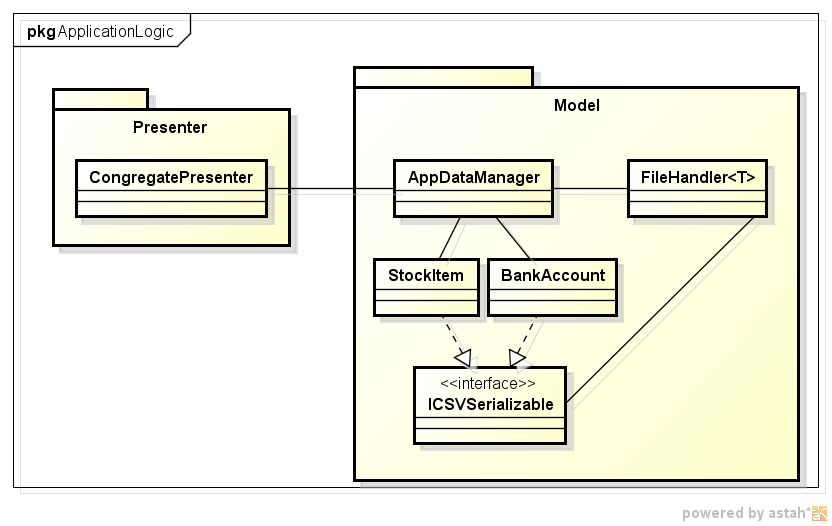
\includegraphics[width=\textwidth]{gfx/application_logic.png}
\caption{Abstract overview of project \texttt{application logic}}
\label{fig:application_logic}
\end{center}
\end{figure}

It can be seen that the \texttt{AppDataManager}-class works as a \textit{facade} for the rest of the model.

Noteworthy implementation in this package are the \texttt{FileHandler} and the realisation of error handling.

\subsection{FileHandler}
\label{subsec:filehandler}

The FileHandler-class utilizes the concept of generics: this way it is possible to reuse this class for multiple classes that need to be persisted.

To allow the serialization and de-serialization-logic to be separated from the file-handling logic, the FileHandler-class requires all classes that need to be persisted to implement the \texttt{ICSVSerializable}-interface:

\lstinputlisting[caption=Interface \texttt{ICSVSerializable}]{\logicRoot/Interfaces/ICSVSerializable.cs}

Due to this fact - both - the \texttt{StockItem} and the \texttt{BankAccount}-class implement this interface.

\subsection{Error handling}
\label{subsec:error_handling}

Error handling is achieved by separate classes called \texttt{ErrorMessageCollection} and \texttt{ErrorMessage}.

On validation errormessages will be added to an errormessagecollection that can be accessed from the presenter to display the occurred errors.

As an example the code of the StockItem's \texttt{Validate()} method, as well as a sequence-diagram of the calling sequence is shown:

\begin{lstlisting}[caption=Validate method of StockItem]
public static bool Validate(String stockCode, String name, String supplierName, double unitCost, int required, int currentStock)
        {
            if (String.IsNullOrEmpty(stockCode) || !IsValidStockCode(stockCode))
            {
                ErrorMessages.Add(new ErrorMessage("Need a stockcode that adheres to the stockcode format: 4 numbers."));
            }
            if (String.IsNullOrEmpty(name))
            {
                ErrorMessages.Add(new ErrorMessage("Need an item name."));
            }
            if (String.IsNullOrEmpty("supplierName"))
            {
                ErrorMessages.Add(new ErrorMessage("Need a supplier name."));
            }
            if (unitCost < 0.0)
            {
                ErrorMessages.Add(new ErrorMessage("Unit costs must be greater or equal 0."));
            }
            if (required < 0)
            {
                ErrorMessages.Add(new ErrorMessage("Required must be greater or equal 0."));
            }
            if (currentStock < 0)
            {
                ErrorMessages.Add(new ErrorMessage("Current must be greater or equal 0."));
            }
            return ErrorMessages.Count == 0;
        }
\end{lstlisting}

\begin{figure}[H]
\begin{center}
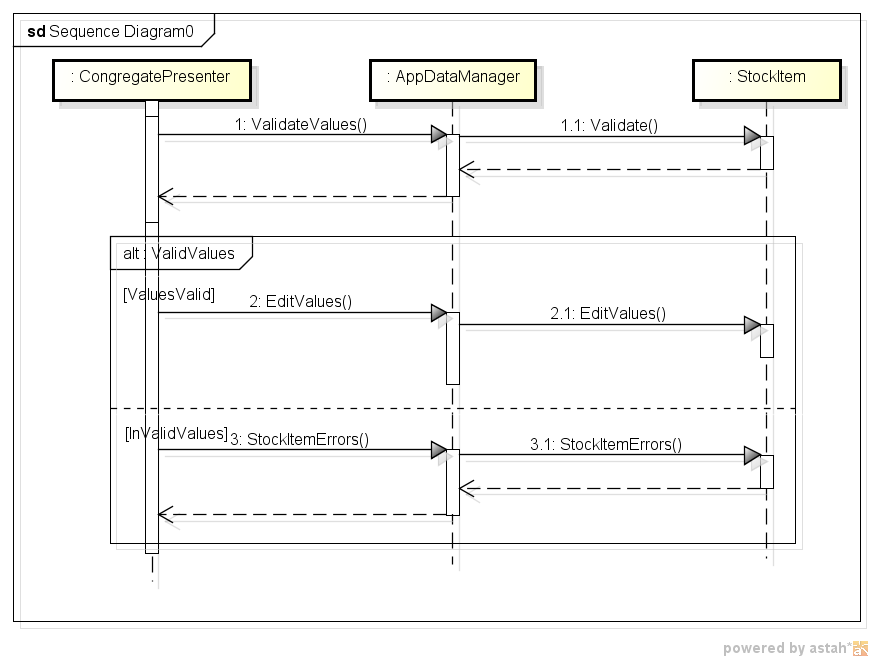
\includegraphics[width=\textwidth]{gfx/error_handling.png}
\caption{Sequence diagram of input validation}
\label{fig:error_handling}
\end{center}
\end{figure}